%
% CHAPTER Versuch 3
%
\chapter{Aufnahme eines Weißbildes}
\label{chap:VERSUCH_3}
Kalibrierung der Sensitivität mit Hilfe eines Weißbildes.
\section{Fragestellung, Messprinzip, Aufbau, Messmittel}
\label{chap:VERSUCH_3_FRAGESTELLUNG}
Im zweiten Teil wurde der Offset eines einzelnen Pixel im Bild mit Hilfe eines Dunkelbildes korrigiert. In diesem Teil der Kalibrierung wird die Sensitivität der Pixel korrigiert. Die Pixel weisen in ihrer Sensitivität ein hohes lineares Verhalten auf. Allerdings ist die Empfindsamkeit der einzelnen Pixel, zu schulden von Fertigungstoleranzen, nicht identisch. Weiter spielt die sogenannte Vignettierung mit in diesen Fehler ein. Bei dieser handelt es sich um ein ungleichmäßiges Ausleuchten der Sensorfläche durch die Optik, so dass an den Sensorrändern weniger Licht auf den Sensor fällt als in der Mitte. Deshalb gilt es auch hier eine Pixelweise Anpassung der Sensitivität vorzunehmen, damit Fertigungstolleranzen und Vignettierung kompensiert werden. Eigentlich müsste man für jede Fokuseinstellung ein eigenes Weißbild aufnehmen. Daher ist die weiße Fläche, die abgelichtet werden soll in gleicher Entfernung, wie das Graukeilbild angebracht. 
Bei der Aufnahme des Weißbildes muss darauf geachtet werden, dass es sich bei der Aufnahmeflache um eine möglichst homogen strukturierte handelt. Diese sollte auch gleichmäßig ausgeleuchtet sein.
Dann müsste theoretisch jeder Pixel den selben Wert haben. Die Praxis zeigt jedoch, dass diese Werte nicht alle gleich sind, da die einen eine höhere Sensitivität haben als andere. Diese Sensitivität entspricht gerade der Steigung einer Geraden, welche ja als Faktor auf die gemessene Größe einwirkt. Um diesen Faktor nun zu korrigieren müssen wir ihn durch den entprechenden Pixelwert des Weisbildes dividieren, um so eine Anpassung der Sensitivität zu erlangen. Da das Bild jedoch auf unbrauchbare weise verändert werden würde, wenn man einfach die korrespondierenden Pixelwerte von Weißbild mit dem Grauwertkeilbild verrechnen würde, muss das Weißbild auf einen Mittelwert von eins normiert werden. Sonst würde der Wert eines Pixels im Weißbild beispielsweise bei 178 liegen und das zu korrigierrende Bild würde drastisch verdunkelt werden. Wird das Weißbild jedoch normiert liegt der Betrag eines Pixelwertes um Eins herum. Dies kann man sich dann als prozentuale Anpassung von der Sensitivität eines Pixels vorstellen. Die Normierung des Weißbildes erreicht man, indem jeder Pixel dessen durch den Mittelwert des gesamten Bildes dividiert wird.
Das Weißbild selbst ist auch wieder von thermischen Rauschen belastet, weshalb wiederum zehn Bilder aufgenommen werden und ein Durchschnittsbild berechnet wird. Von diesem wiederum wird das Dunkelbild abgezogen, um den Offset der einzelnen Pixel zu korrigieren. Anschließend kann das Weißbild normiert werden.
Dann kann das Graukeilbild durch das Weißbild dividiert werden, wobei eine Pixelweise Division darunter verstanden wird.

\section{Messwerte}
\label{chap:VERSUCH_3_MESSWERTE}
\begin{figure}[H]
\centering
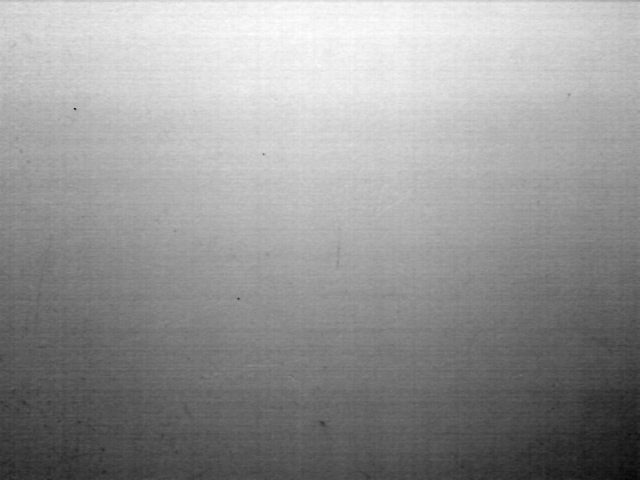
\includegraphics[width=150mm]{weissbildMean_maximiert.png}
\caption{Weißbild \textit{(Mittelwert der Zehn)} Kontrastmaximiert}
\label{img:WeissBild_KontrastMax}
\end{figure}
\section{Auswertung Interpretation}
\label{chap:VERSUCH_3_AUSWERTUNG}
Das kontrastmaximierte Weißbild \ref{img:WeissBild_KontrastMax} ist in der oberen Hälfte im Vergleich zur unteren insgesamt heller. Dies hängt damit zusammen, dass das Bild an einem Fenster aufgenommen wurde und das rein scheinende Licht diese Seite wohl stärker ausgeleuchtet hat. Trotz der höheren Helligkeit im oberen Bild ist die Vignettierung zu erkennen. Diese sieht man vor allem in den Ecken des Bildes. Die schwarzen Flecken im Weißbild sind nicht als Deadpixel zu deuten. Diese sind lediglich auf eine inhomogene Oberfläche zurückzuführen\textit{(Schmutz)}.